\section{Background}

Mobile devices and high-speed internet have dramatically changed the way the people can view video media. In this section, we'll first discuss the popularity of different methods of watching video media, including via mobile devices, and how modern methods have affected how people view video advertisements. We'll then discuss how streaming video over internet opens up opportunities for granular targeting of video media, including advertisements and TV shows. 

Following on from this, we give an overview of research in viewer engagement in these methods of watching video media. We discuss how targeting particular video towards users can improve this, leading us to discuss programme recommendation as a way to facilitate this. We review current research in interactive video media, specifically in the context of improving viewer engagement \cite{what_is_engagement}. We then summarise the availability of statistics to advertisers before finally considering the costs of streaming services, focusing on individualised services.

\subsection{History and recent trends of video advertising}

	Live television channels, such as Channel 4, and streaming services, such as Youtube\footnote{Youtube video streaming website -- \footurl{www.youtube.com}}, display programme content with video advertisements apportioned amongst this content at both regular intervals, and between distinguishable items of content. These advertisements typically vary in subject and style in a number of ways in order to increase the efficiency of the advert by maximising the size of the captured audience who fit the target audience for the given advert.

	Television broadcasts typically have very low granularity - as they are, by their nature, viewed simultaneously by everyone who is watching a particular channel. This leaves a limited amount of factors for advertisers to maximise their efficiency. These factors include the time of day; the adjacently showing content; the typical target audience of the channel; and location at a very broad scope (regions, e.g. East Midlands).

	% Advertisers like targetting
	A technical report released by \citet{brightroll-report} discusses video advertising statistics. In 2012, 53\% of advertisers cited targeting as the most valuable aspect of online video. Online video typically boasts significantly more factors to target upon, including browsing history (behavioural data), user demographics and interests amongst others. On the contrary, in 2012 advertisers expressed a 41\% drop compared to the previous year in the important of reach (size of audience). This can be attributed to an increased confidence that online video has a large enough audience, which in turn emphasises the importance on targeting specific audiences. This is emphasised by 35\% of advertisers agreeing that demographics data is the most valuable form of targeting -- the largest targeting type in comparison to others such as contextual and geographic.

	% Highly useful google research areas: http://www.google.co.uk/adwords/watchthisspace/benchmarks-and-insights/
	% They like good pricing models

	Google, a leader in online advertising, has reinforced this shift in ideology towards targeted video by supporting a ``Cost Per View'' (CPV) pricing strategy. Cost per view differs from cost per impression (CPI) in that pricing is based upon users who choose to watch a video instead of video that is simply passively playing. This strategy can also incorporate advert skipping. YouTube, a Google product, offers ``TrueView''\footnote{Google Insights: Online Video -- \footurl{http://www.google.co.uk/adwords/watchthisspace/benchmarks-and-insights/online-video/} (Accessed: 04/12/2012)} which only charges an advertiser if the viewer reaches the end of the advert without using a skip button. This is an attractive option for advertisers, as TV advertising does not return any metrics to identify who out of the audience reach is engaged by the advertisement.

	% Advertisers need people to be engaged in their adverts
	\citet{three-screen} reports a growing trend in which viewers choose the best medium (television, online and mobile) available to them to consume content according to the viewers perception of the quality of the content and its availability. 31\% of internet activity occurs when consumers are also watching television in domestic environments. A growing number of households are adopting Digital Video Recorder (DVR) technology, with 29\% of US homes able to time shift television which allows viewing only content the viewer is interested in, including the skipping of adverts \citep{gal2006targeted}. However, live TV viewing still accounts for the majority of video consumption, but is growing at a slower rate than the richer online platforms.

	More advanced time-shifting systems such as TiVo\footnote{TiVo -- \footurl{http://www.tivo.com/}} allow users to pause and rewind live TV. It achieves this by recording a rolling 30 minutes of the last two channels the user was watching\footnote{Description of TiVo's Live TV rewinding technology -- \footurl{http://www.mytivo.com.au/whatistivo/tivois/pauserewind/}}. While this improves the user experience by reducing the likelihood they will miss the start of a show, the two channel limitation reduces the usefulness of these systems in terms of user experience. Additionally, while watching a time-shifted channel, a user may fast-forward. This may be seen as an opportunity to skip through adverts, negatively affecting advertisers.

	% Here comes rich video!
	The introduction of online video and touch mobile devices has introduced opportunities for novel interactivity which can not exist on TV. Online advertisements have long used animated images and flash technology to introduce this level of interactivity to computer users. Recent developments in web standards such as HTML5 have given rise to rich video \citep{HLS}. Rich video allows supplementary out-of-band metadata (information separate to the video itself) in videos and the opportunity for viewers to manipulate aspects of videos. 

	For example, YouTube allows content owners to annotate their videos with extra clickable information at specific points in time, as shown in Figure~\ref{fig:youtube_annotation}. A study by advertising network DoubleClick highlighted how this form of user engagement can increase advert efficiency, revealing ``Rich Media with Video'' to be the best choice for brand awareness, brand favour and purchase intent \citep{rich-video}. This rich interaction between the user and the device allows for advertisers to design fun, memorable and informative interactions into their adverts, and collect consequential user information through the audience to advertiser information flow.

	\begin{figure}[htb]
		\centering
			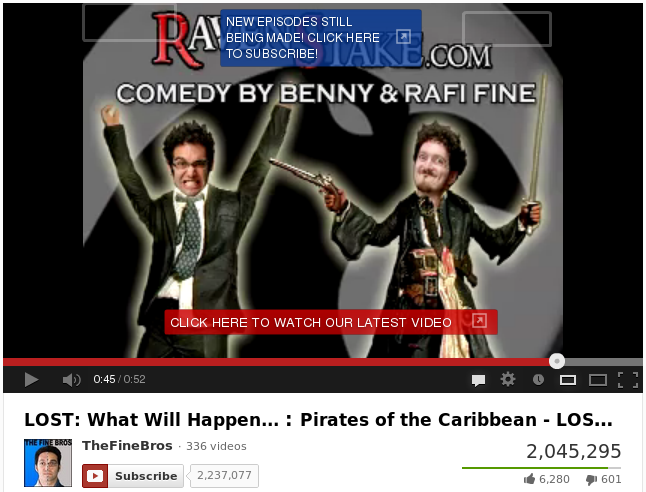
\includegraphics[width=0.6\textwidth]{images/youtube_annotations.png}
		\caption{YouTube video showing annotations overlaid (in blue and red)}
		\label{fig:youtube_annotation}
	\end{figure}

	% Stats
	Traditional TV viewing statistics are not immediate or accurate due to the lack of feedback directly from the viewing device. This information is usually obtained by surveying small samples of viewers using the ``Nielsen Rating'' system \citep{nielsen-sample}. Because the Nielsen system is an opt-in study, the sample is non-random in that all participants who take part are those individual who chose to opt in, introducing flaws into any results obtained. This sample is also extremely small at approximately 37,000 homes in the USA which accounts for less than 0.5\% of the population \citep{nielsen-sample}. In contrast to traditional TV, online platforms allow immediate return of accurate statistics such as click through rates and viewer demographics. Advertisers consider better metrics to be the most important factor on encouraging higher digital video advertising spend \citep{brightroll-report}.

	%The main broadcasters -- BBC, Channel~4, ITV -- have made available on-demand services for tablet computers, which allows users to watch programmes that have been shown in the past. However, these broadcasters have not made their live streams accessible, which must instead be accessed via a third party app, such as TVCatchup\footnote{TVCatchup on iTunes -- \footurl{https://itunes.apple.com/gb/app/tvcatchup-live-tv/id427900675?mt=8}}.

	%The iPad and other tablet devices have for some time had apps like 4oD available which allows on demand streaming of recorded television content. However the main UK channels have limited provision for \textit{live streaming}.% Channel 4 provided a Paralympics app\footnote{The official Channel 4 Paralympics Real-time Commentary App\url{https://itunes.apple.com/gb/app/channel-4-paralympics/id554157549}} which promised live commentary. Unfortunately this only provided short videos (lacking sound) and text commentary with images much like a Twitter stream or blog.

	%The BBC iPlayer mobile app for devices such as the iPad provides a limited subset of its live TV channels and Sky subscribers can use Sky Go to get a similarly restrictive subset of the Sky channels. This limited uptake by large broadcasters is surprising considering statistics such as those shown by \citet{viacom} and that \citep{socialTVPaper} presents strong evidence that tablets are becoming a major portal for television viewing. This has however allowed several third parties are taking advantage of this market gap such as \footnote{TVCatchup Live TV App: \footurl{http://www.tvcatchup.com/}}.

	%Traditional costings analysis methods such as the Spence-Owen analysis of pay TV assumes that the cost of adding another viewer is \$0.00 \citet{broadcastEconomics}. For traditional radio broadcast this is clearly the case as the radio waves are pervasively broadcast and to receive the signal a user needs only have an antenna to detect the waves, there is nothing sent back to the broadcaster, hence no additional load. Therefore to enable broadcasters to economically transmit television over the Internet the amount of communications each user makes with a broadcaster owned server should be minimised as every communication to a broadcaster owned server increases the server load meaning that more must be invested in server technologies to handle the load as usage increases.

	\subsubsection{Mobile video}

		\citet{mobile-planet} reveals that smartphone usage in the UK is rising rapidly -- as of 2012, 51\% of the UK population owns a smartphone device. As mobile advertising is a strong growth industry, it is of interest to content owners to expose their products and services on this platform. By the pervasive nature of mobile devices, more users are relying on their smartphone outside of the home in order to research and purchase products; watch video; communicate and to stay informed. This report further indicates that 66\% of smartphone users watch video on their device and 84\% of users notice mobile ads while using their phone. 

		These two factors together present an opportunity for content owners to engage users with their services by employing the use of rich video with advertising. With over 31\% of advertisers considering mobile video as the area in which advertising spend will increase most \citep{brightroll-report}, TV broadcasters need to shift towards a more engaging platform.

\subsection{Advert engagement}

	User engagement is defined by \citet{what_is_engagement} as a user experience consisting of \textit{``challenge, positive affect, endurability, aesthetic and sensory appeal, attention, feedback, variety/novelty, interactivity and perceived user control''}. \citet{advert_engagement} describes a study performed, showing that user engagement is important for advertisements to be effective, and that advert relevance boosts this engagement. Both \citet{advert_engagement} and \citet{yahoo-intrusive-advertising} report finding that advert relevance positively correlates with user experience and performance, indicators of engagement \citep{what_is_engagement}, which is backed up by \citet{plummer2006measures}, who describes a lack of relevance reducing engagement.

	Engagement cannot be measured directly, but can be inferred from other measurements. \citet{time_perception} report that time perception correlates well with engagement, and may be used as a measurement. Information recall is used in the study described in \citep{advert_engagent} as an indicator of user engagement, and correlates with attention \citep{interactions_attention_memory}, a requirement for engagement \cite{what_is_engagement}.

\subsection{Targeting}

	\citet{yahoo-intrusive-advertising}
	* time perception, known to indicate engagement
	* relevance shown to influence user experience

	\citet{nettelhorst2012effects}
	* adverts that are relevant to users are more likely to be engaging to a viewer

	\citep{interactions_attention_memory}
	* information recall, known to correlate with attention

	\citep{davidson2012}
	* YouTube does targeting through a recommender system. Accounts for 60\% of video clicks

	\citep{gal2006targeted}
	* skipping

	ad breaks positioned early in a programme are more effective \citep{jeong2011position}

\subsection{Programme recommendation}
	
	PREVIOUS WORK \citep{personalisedEPG}

	% What are they? Are they used?
	Recommendation systems---systems which recommend unseen items to users based off relevant data---are a mature area of research, with a huge number of industrial implementations existing to back up a large theoretical base. Recommendation systems are widely used in internet streaming media services, including YouTube, 4od\footnote{Channel 4 On Demand -- \footurl{http://www.channel4.com/programmes/4od}} and iPlayer\footnote{BBC iPlayer -- \footurl{http://www.bbc.co.uk/iplayer}}, and can be of enormous commercial value; evidence of this is given by the US\$1,000,000 2009 Netflix prize awarded to Pragmatic Chaos for improving upon Netflix's movie recommendation algorithm Cinematch, in return for granting Netflix a non-exclusive licence \citep{pragmatic_chaos}.

	% Collaborative/content-based filtering
	Two distinct approaches of recommendation system exist; collaborative-filtering and content-based filtering. Collaborative-filtering approaches attempt to build a profile of user behaviours, and recommend items which users with similar profiles have positively rated. This approach requires no data on the actual items being recommended, but requires collection of user preference data. As an example, a collaborative-filtering based programme recommender may recommend programmes to a user which similar users (users who have similar rating profiles to the user being recommended to) have rated highly, but the user has not yet seen. Content-based filtering requires information on the items, where items are recommended to a user which are similar to those which the user has positively rated in the past. The quality of recommendations weighs heavily on the quality of the item information available. An example content-based filtering programme recommender may give each programme a set of genres, and recommend programmes to a user which have similar genre sets as those they have rated highly.

	% Implicit data collection methods.
	To recommend programmes to a user, user preference data is used to construct a user preference model, from which new programmes are compared against. This preference data is often obtained through explicitly asking the user for programme ratings; while this is sufficient information to learn a users preferences, the user is required to halt their workflow to provide a rating \citep{implicit_indicators}, which may be seen as an additional chore with no immediate apparent reward. This lack of perceived benefit can lead to users being unwilling to provide explicit programme ratings \citep{8_challenges}, meaning a recommender system has no information from which to improve. In addition, explicit ratings are prone to biases from user subjectivity, item popularity and rating habits \citep[p.~304]{recommender-systems-handbook}. Collecting ratings implicitly combats this, which may be done for any detectable user interaction, sequence of interactions, or lack thereof \citep{implicit_indicators}, assuming that it correlates with user preferences.

	% Cold-start problem.
	Certain recommendation system implementations are faced with the cold start problem \cite{cold-start-problem}, which is the problem of the recommender being unable to give high-quality recommendations on items for which sufficient information has not yet been gathered. In a live TV recommendation system, at the point when a TV show is recommended to users it has not yet been aired and therefore cannot use collaborative data to recommend the programme. After airing, the show may pick up many viewer ratings, but in a system that deals only with live TV, these ratings are now useless as the programme will not be shown and hence not have the chance to be recommended again. New users also present a cold-start problem, as they start with no rating data from which to base recommendations. Designing recommender systems to deal with the cold start problem is an active area of research; \citep{cold-start-problem} have shown that that certain machine-learning methods are more able to learn from sparse data than others, despite having lower prediction accuracy with dense data, and hence switching technique depending on the density of data available may outperform a single algorithm . Approaches which combine both user rating information (collaborative data) and item information (content data) have been developed \citep{generative_models}, which can use content data as an initial source of information from which early recommendations may be based, and improve recommendations once collaborative data becomes available.

	Research is being performed into the extension of programme recommenders into advertisement recommenders \citep{contextual_advertising}. While similar algorithms are used, advert recommenders have a different set of considerations in providing optimal adverts: who is watching, what is being watched, programme popularity and business rules (e.g., the amount paid for the advertisement) \citep{contextual_advertising}.

\subsection{Interactive television}

	Television is already switching to become an interactive platform; the 2012 live election debate was augmented with live twitter streams, discussed by \citep{2010_election}, and the 2012 olympic games was given an online interactive video player\footnote{Interactive 2012 Onlympics video player -- \footurl{http://www.bbc.co.uk/sport/olympics/2012/live-video}}. \citet{tv_stb_overview} gives an overview of the state of interactive TV set-top box development, and describes a rapidly growing market in Europe and Asia. A number of problems in standardization, network architecture and upgradability are described, but many of these become redundant upon removal of the assumption that interactive TV requires a set-top box, and instead assuming the software runs on a personal computer communicating via the internet.

	Relating to interactive idvertisement, \citet{integrated-approach-advertising} discusses a number of issues including that of timing when the user decides to interact with the advert. When interacting with an advert which requires more time than the length of the advert, it is undesirable to halt the interaction and switch to the next advert. However, the alternative means overrunning into the time in which the subsequent adverts or even the main programme would be broadcasting, which raises a number of issues, particularly if the stream being viewed is live. The solutions given are to either record the stream being missed, or to minimise the interaction time required with one of the following techniques:
	\begin{itemize}
		\item Interaction in which the user requests to be contacted at a later point in time, which could be through email, a phone call, a visit, a letter or any other contact method.
		\item Interaction in which the user `bookmarks' the interactive content, which may be returned to at a later point in time.
		\item Split the screen into two partitions; one showing the main programme flow and the other containing the interactive advertisement content. 
	\end{itemize}

	% use of interactivity in tv and advertising
	\citep{integrated-approach-advertising}

	% use of social media in tv
	% See TriggerTV: Exploiting Social User Journeys within an Interactive TV System

	\citet{informationOverload}

	Research has shown that \citet{humanVariables}
	
	studies of interactivity on websites described in \citet{Teo2003281}

\subsection{Advertiser statistics and analytics}
	% Low granularity: TV regions, few people use a box that transmits usage data
	% High granularity: YouTube, Google Analytics

\subsection{The cost of streaming}
	Whenever a new service is provided, there will be an initial cost to the provider, to install any hardware and create and necessary software. In traditional broadcast economics \citep{broadcastEconomics} the cost of adding users to a service is \$0.00 but with individualised streams this is not the case. Even so, with the considerable number of people now using tablet devices for their TV viewing it seems odd that no major broadcasters have provided their service on these devices. Especially when we consider the prevalence of on-demand services despite the relative costs behind typical implementations of these. When we examine typical unicast-based implementations of on-demand services, it becomes clear that for scalable \textit{live streaming} a new approach is needed.

	Most traditional streaming services provide a unicast stream to each viewer which means that the load placed on the servers increases linearly resulting in a linear increase in costs as more users connect. \citet{cachedStream} realised that this does not scale well and proposes a different architecture using self organising caches and stream segmentation, this type of approach is considered as the standard solution and is further examined by \citet{segmentProxyCaching}. \citet{cachedStream} concludes that their proposed helper decreases load significantly so using a system such as that proposed with a protocol such as Apple's HLS\cite{HLS} which segments the stream as part of the protocol the cost of adding a user can be significantly reduced however it still does not meet the zero requirement noted in \citep{broadcastEconomics}.

	Another internet broadcast possibility is using multicast technology\citep{multicast}. Multicasting reduces server load significantly as the source need only forward the stream to one endpoint -- the multicast group. This means that adding new listeners does not negatively impact server performance hence giving zero additional cost required for the Spence-Owen analysis\citep{broadcastEconomics}.

	While mobile device usage continues to rise, development by major broadcasters for this platform is slow. As many of the main channels provide on-demand services such as Channel 4's 4oD. The costs of unicast services mean that expansion into this new area must be proven economically viable. Systems such as Project4 attempt to improve the viability by replacing the adverts with ones targeted towards their more specific user demographic of students while keeping costs low using multicast technology. By extending this idea of improved targeting we can infer that by providing an app which could give individual granular targeting it seems likely that advertisers would be able to reach a greater percentage of their target audience with less advert showings. Unfortunately, this would require reverting to unicast for at least the adverts as each user's stream would be different.

	A hybrid approach, using multicast where possible, to minimise unicast traffic, would minimise the cost of such a granular service to broadcasters while keeping the granularity which would be highly valued by advertisers. Additionally, using an easily cacheable segmenting protocol such as HLS \citep{HLS}, with a helper such as that proposed in \citep{cachedStream} individual customisation could be maximised while minimising server load and hence costs making this sort of system economically viable.
